\chapter{Dynamics of the snow cover} \label{chap:snow}
\renewcommand{\tabdir}{chapters/part_processes/snow/tab}
\renewcommand{\figdir}{chapters/part_processes/snow/fig}

%%%%%%%%%%%%%%%%%%%%%%%%%%%%%%%%%%%%%%%%%%%%%%%%%%%%%%%%%%%%%%%%%%%%%%%%%%%%%%%%
%%%%%%%%%%%%%%%%%%%%%%%%%%%%%%%%%%%%%%%%%%%%%%%%%%%%%%%%%%%%%%%%%%%%%%%%%%%%%%%%
%%%%%%%%%%%%%%%%%%%%%%%%%%%%%%%%%%%%%%%%%%%%%%%%%%%%%%%%%%%%%%%%%%%%%%%%%%%%%%%%

\section{Energy balance method} \label{sec:snow-enBal}

%%%%%%%%%%%%%%%%%%%%%%%%%%%%%%%%%%%%%%%%%%%%%%%%%%%%%%%%%%%%%%%%%%%%%%%%%%%%%%%%
%%%%%%%%%%%%%%%%%%%%%%%%%%%%%%%%%%%%%%%%%%%%%%%%%%%%%%%%%%%%%%%%%%%%%%%%%%%%%%%%

\subsection{Capabilities and limitations} \label{sec:snow-enBal_caps-lims}

In many catchments, snow storage and melting are important components of the water cycle. Snow melt, possibly accompanied (or caused) by rainfall is a major cause of flood generation in many catchments. However, the structure of a natural snow cover is very complex and the simulation of its dynamics is difficult. Therefore, any snow model is subject to a number of simplyfing assumptions and limitations. The most important limitations of the snow model described in this section are:

\begin{itemize}
  \item The snow pack is treated as homogeneous (well mixed) layer. Thus, possible stratification is neglected.
  \item Shortwave radiation is not corrected for slope and aspect, \ie{} the model should be applied only to horizontal surfaces or larger areas where the effects of slope and aspect may be assumed to level out.
  \item The current model does not account for vegetation cover. In reality, vegetation may affect the snow dynamics in many ways (\eg{} due to interception, sheltering, shadowing, long-wave emission, etc.).
\end{itemize}

\subsection{Basics of the energy balance method} \label{sec:snow-enBal_basics}

\subsubsection{State variables}
A physically-based simulation of the snow dynamics requires the water equivalent and the energy content of the snow pack to be considered as state variables \citep[\eg][]{Dyck1995,Tarboton1996}. In the model described here, the snow albedo is introduced as an auxiliary state variable.

\paragraph{Snow water equivalent} The snow water equivalent, \snowWaterEquivalent{} (m), represents the total volume of water (stored in solid and liquid form) contained in a snow pack covering an area of 1~\sqm. \snowWaterEquivalent{} is defined by \eqnref{eqn:snow-enBal_defSWE}
\begin{equation} \label{eqn:snow-enBal_defSWE}
	\snowWaterEquivalent = \snowHeight \cdot \frac{\densitySnow}{\densityWater}
\end{equation}
  
where \snowHeight{} is the snow height (m) and \densitySnow{} and \densityWater{} represent the densities of snow and water (kg/\cbm{}). The unit of \snowWaterEquivalent{} or the snow height (meters) is equivalent to \cbm/\sqm. To convert from units of m to units of kg/\sqm{}, one has to multiply \snowWaterEquivalent{} with the density of \emph{water} \densityWater{} in kg/\cbm{} (even though a part or all of the stored water is in solid form).

\paragraph{Energy content} The energy content, \snowEnergyContent{} (kJ/\sqm{}), represents the energy stored in the snow pack. \snowEnergyContent{} is defined relative to a reference energy content (\snowEnergyContent= 0 for ice at 0\celsius) as detailed below.

\paragraph{Snow albedo} The snow albedo \snowAlbedo{} (--) represents the reflectivity of the snow surface for shortwave radiation. At each snowfall event, the snow surface is re-born and the albedo is reset to its maximum value associated with freshly fallen snow.

\subsubsection{Processes}
The dynamics of \snowWaterEquivalent{} is described by the mass balance and the dynamics of \snowEnergyContent{} is controlled by the energy balance. Both mass and energy balance are coupled as illustrated in \figref{fig:snow-enBal_snow-fluxes}. A simulation of the state variables therefore requires a simultaneous solution of  differential equations summarized in \tabref{tab:snow-enBal_processmatrix} using a matrix notation.

\begin{figure}[htb]
  \centering
  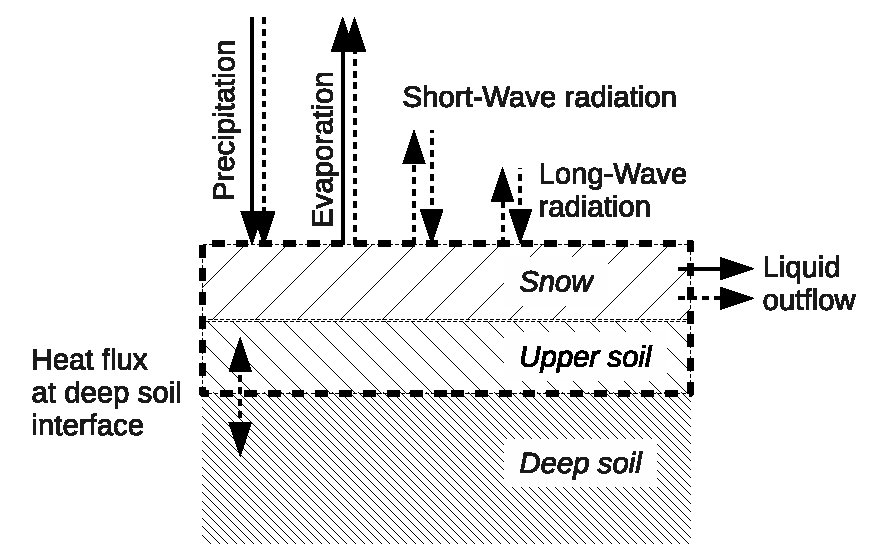
\includegraphics[width=0.48\textwidth]{\figdir/snow-fluxes.eps}
  \caption[Fluxes of mass and heat to be considered when simulating the snow dynamics.]{Fluxes of mass (solid arrows) and heat (dashed arrows) to be considered when simulating the snow dynamics. \label{fig:snow-enBal_snow-fluxes}}
\end{figure}

\begin{table*}
  \caption[Process matrix of the energy balance snow model.]{Process matrix of the energy balance snow model describing the dynamics of the state variables. The rate expressions containing state variables, forcings, and parameters are derived in \secref{sec:snow-enBal_fluxrates-energy} \& \ref{sec:snow-enBal_fluxrates-mass}. The stoichiometry factors \stoifacPrecMassToEnergy, \stoifacSublMassToEnergy, and \stoifacFlowMassToEnergy{} (kJ/\cbm) used to convert between mass and energy are derived in \secref{sec:snow-enBal_mass-energy-relations}. The $(+)$ indicates that precipitation has an impact on the albedo but this is considered a separate process called 'Albedo evolution' (see \secref{sec:snow-enBal_albedo}). \label{tab:snow-enBal_processmatrix}}
\begin{tabularx}{\textwidth}{|X|ccc|rr|} \hline
\rowcolor[gray]{0.9}
                  &  \multicolumn{3}{>{\columncolor[gray]{0.9}}c}{\textbf{Stoichiometry factors}}      &      &         \\
\rowcolor[gray]{0.9}
\textbf{Process}  & \snowEnergyContent & \snowWaterEquivalent & \snowAlbedo & \textbf{Rate expr.} & \textbf{Rate units} \\
\rowcolor[gray]{0.9}
                  & (kJ/\sqm)          & (m)                  & (--)        &                     &                     \\ \hline

Short-wave radiation balance & $0.001$ & $0$ & $0$ & \netRadiationShort & W/\sqm \\
Long-wave radiation balance  & $0.001$ & $0$ & $0$ & \netRadiationLong & W/\sqm \\
Soil heat flux               & $0.001$ & $0$ & $0$ & \heatfluxSoil & W/\sqm \\
Sensible heat flux           & $0.001$ & $0$ & $0$ & \heatfluxSens & W/\sqm \\
Precipitation                & $\stoifacPrecMassToEnergy$ & $1$ & $(+)$ & \massfluxPrec & m/s \\
Sublimation                  & $-\stoifacSublMassToEnergy$& $-1$ & $0$ & \massfluxSubl & m/s \\
Melt water outflow           & $-\stoifacFlowMassToEnergy$ & $-1$ & $0$ & \massfluxFlow & m/s \\
Albedo evolution             & $0$     & $0$ & $1$ & \albedoChangeRate & 1/s \\ \hline
\end{tabularx}
\end{table*}

\subsubsection{Definition of the energy content} \label{sec:snow-enBal_energy-content}
The energy content of the snow cover, \snowEnergyContent, can only be defined with respect to some reference. A useful reference state is ice at a temperature of 0\celsius{} for which \snowEnergyContent{} is zero by convention \citep{Tarboton1996}. With that reference, the relation between the energy content \snowEnergyContent{} and the (average) snow temperature \snowTemperature{} follows from the considerations below:

\begin{enumerate}

  \item Negative values of \snowEnergyContent{} indicate that \snowWaterEquivalent{} consists of solid water only and the snow temperature is negative. The relation between temperature and energy content is then determined by the heat capacity of the ice mass according to \eqnref{eqn:snow-enBal_heating-of-ice} (see \tabref{tab:snow-enBal_constants} for definition of symbols).
  \begin{equation} \label{eqn:snow-enBal_heating-of-ice}
    \frac{d\snowTemperature}{d\snowEnergyContent} = \frac{1}{\snowWaterEquivalent \cdot \densityWater \cdot \specHeatIce}
  \end{equation}

  With respect to the energy content, it is useful to treat the snow cover and the upper soil up to a certain depth \soilInteractionDepth{} as a single system (dashed box in \figref{fig:snow-enBal_snow-fluxes}). The upper soil is defined as the layer which thermally interacts with the snow cover on short time scales. Then, \eqnref{eqn:snow-enBal_heating-of-ice} expands to \eqnref{eqn:snow-enBal_heating-of-ice-soil-system}, where \soilInteractionDepth{} (m) represents the depth of the upper soil, \densitySoil{} (kg/\cbm) is the soil density and \specHeatSoil{} (kJ/kg/K) is the soil's specific heat capacity.
  \begin{equation} \label{eqn:snow-enBal_heating-of-ice-soil-system}
    \frac{d\snowTemperature}{d\snowEnergyContent} = \frac{1}{\snowWaterEquivalent \cdot \densityWater \cdot \specHeatIce + \soilInteractionDepth \cdot \densitySoil \cdot \specHeatSoil}
  \end{equation}

  Then advantage of treating the snow cover and the upper soil as a single system is that the soil energy flux reduces to the long-term average flux at the interface between shallow and deep soil (see \figref{fig:snow-enBal_snow-fluxes}). This flux is much less variable and may be approxiamed by a constant.

  \item If \snowEnergyContent{} is zero, the temperature is 0\celsius{} and the snow cover still does not contain liquid water as a consequence of the chosen reference.

  \item At positive values of \snowEnergyContent{}, some fraction of \snowWaterEquivalent{} exists in liquid form. As long as ice and liquid water coexist, the snow temperature remains at 0\celsius{} and all energy input is consumed by the melting process. The energy required to completely melt a snow cover at a temperature of 0\celsius{} which consists of solid water only is determined by the ice's heat of fusion (see \tabref{tab:snow-enBal_constants}) and equals (\eqnref{eqn:snow-enBal_melting-of-ice}):
  \begin{equation} \label{eqn:snow-enBal_melting-of-ice}
    \snowWaterEquivalent \cdot \densityWater \cdot \fusionHeatIce
  \end{equation}

  \item There is a critical value of \snowEnergyContent{} where all ice was melted and only liquid water is left. The snow has ceased to exist. If more energy is input, the temperature of the liquid water rises above zero according to \eqnref{eqn:snow-enBal_heating-of-water} (see \tabref{tab:snow-enBal_constants} for definition of symbols).
  \begin{equation} \label{eqn:snow-enBal_heating-of-water}
    \frac{d\snowTemperature}{d\snowEnergyContent} = \frac{1}{\snowWaterEquivalent \cdot \densityWater \cdot \specHeatWater}
  \end{equation}
\end{enumerate}

Based on these considerations, the relation between \snowEnergyContent{} and \snowTemperature{} can be computed for a snow cover with a given \snowWaterEquivalent{} as illustrated in \figref{fig:snow-enBal_energy-temperature-relation}.

\begin{figure}[htb]
  \centering
  \includegraphics[width=0.48\textwidth]{\figdir/snow-energy-temperature.eps}
  \caption[Relation between energy content and temperature for a sample snow cover.]{Relation between energy content and temperature for a sample snow cover with \snowWaterEquivalent= 0.05~m (soil interaction not taken into account). The thin vertical dashed line marks the (theoretical) energy content when the snow cover consists of liquid water only, \ie{} when all ice was melted. \label{fig:snow-enBal_energy-temperature-relation}}
\end{figure}

With the basic relations given by \eqnref{eqn:snow-enBal_heating-of-ice}--\ref{eqn:snow-enBal_heating-of-water} we can infer from the energy content \snowEnergyContent{} two important variables: the temperature \snowTemperature{} of the snow pack and the dimensionless fraction of liquid water \snowFractionLiquid.

\begin{table}[htb]
  \caption[Snow-related physical constants.]{Snow-related physical constants \citep{Tarboton1996,Dyck1995}. \label{tab:snow-enBal_constants}}
  \begin{tabularx}{0.48\textwidth}{|p{0.07\textwidth}rrX|} \hline
     \rowcolor[gray]{0.9}
     \textbf{Symbol}   & \textbf{Value}  & \textbf{Unit}    & \textbf{Description} \\ \hline
     \densityIce       & $\approx$922  & kg/\cbm & Density of ice \\
     \specHeatIce      & 2.09  & kJ/kg/K & Specific heat of ice \\
     \fusionHeatIce    & 333.5 & kJ/kg   & Latent heat of ice fusion (melt heat) \\
     \sublimHeatIce    & 2837  & kJ/kg   & Latent heat of ice sublimation (=\fusionHeatIce+\evapHeatWaterZero) \\
     \densityWater     & 1000  & kg/\cbm & Density of water \\
     \specHeatWater    & 4.18  & kJ/kg/K & Specific heat of water\\
     \evapHeatWaterZero & 2503  & kJ/kg & Latent heat of water evaporation at 0\celsius \\ \hline
  \end{tabularx}
\end{table}

\subsubsection{Snow temperature}
As the snow temperature is not simulated explicitly, it needs to be inferred from the state variables. Since snow is a good isolator, the snow surface temperature, \snowSurfaceTemperature{}, is generally different from the depth-averaged snow temperature \snowTemperature{} \citep{Tarboton1996}.

\paragraph{Depth-averaged temperature} Since the snow pack is assumed to be homogeneous, only the depth-averaged value, \snowTemperature{}, is directly accessible through the state variables \snowEnergyContent{} and \snowWaterEquivalent. Three cases need to be distinguished (see \secref{sec:snow-enBal_energy-content} for definition of \soilInteractionDepth{}, \densitySoil{} and \specHeatSoil{}):

\medskip\emph{Case 1: } ($\snowEnergyContent < 0$)
\begin{equation} \label{eqn:snow-enBal_energy-temperature-relation-allSolid}
  \snowTemperature= \frac{\snowEnergyContent}{\snowWaterEquivalent \cdot \densityWater \cdot \specHeatIce + \soilInteractionDepth \cdot \densitySoil \cdot \specHeatSoil}
\end{equation}

\medskip\emph{Case 2: } ($0 < \snowEnergyContent < \snowWaterEquivalent \cdot \densityWater \cdot \fusionHeatIce$)
\begin{equation} \label{eqn:snow-enBal_energy-temperature-relation-solidAndLiquid}
  \snowTemperature= 0
\end{equation}

\medskip\emph{Case 3: } ($\snowEnergyContent > \snowWaterEquivalent \cdot \densityWater \cdot \fusionHeatIce$)
\begin{equation} \label{eqn:snow-enBal_energy-temperature-relation-allLiquid}
  \snowTemperature= \frac{\snowEnergyContent - \snowWaterEquivalent \cdot \densityWater \cdot \fusionHeatIce}{\snowWaterEquivalent \cdot \densityWater \cdot \specHeatWater + \soilInteractionDepth \cdot \densitySoil \cdot \specHeatSoil}
\end{equation}

The equation for the first case (\eqnref{eqn:snow-enBal_energy-temperature-relation-allSolid}) directly follows from \eqnref{eqn:snow-enBal_heating-of-ice-soil-system} by multiplying with a negative $\Delta$\snowEnergyContent. The resulting temperature \snowTemperature{} is negative.

The conditions when \eqnref{eqn:snow-enBal_energy-temperature-relation-solidAndLiquid} must be used (second case) follow from the definition of \snowEnergyContent{} and \eqnref{eqn:snow-enBal_melting-of-ice}.

The third case (\eqnref{eqn:snow-enBal_energy-temperature-relation-allLiquid}) is considered here only for completeness since in represents the case where all snow became liquid, and \snowTemperature{} actually represents a water temperature.

\paragraph{Surface temperature} To compute energy fluxes across the snow-atmosphere interface (outgoing long wave radiation, exchange of sensible heat, etc.), an estimate of the surface temperature \snowSurfaceTemperature{} is required.

For estimating \snowSurfaceTemperature{}, \citet{Tarboton1996} assume that the energy fluxes at the snow surface are in equilibrium. \snowSurfaceTemperature{}, which controls some of the flux rates, is determined iteratively as the surface temperature where all energy fluxes balance. They also introduce a tuning parameter (snow surface conductance).

To avoid iteration, the very simple approach presented in \eqnref{eqn:snow-enBal_surfaceTemperature} is used here to estimate \snowSurfaceTemperature{}. Therein, \airtemp{} (\celsius) is the air temperature and $\mu$ is a weighting parameter. If $\mu=0$, the surface temperature \snowSurfaceTemperature{} is taken to be equal to the depth-averaged temperature \snowTemperature{} and if $\mu=0.5$, the surface temperature is simply computed as the mean of \snowTemperature{} and \airtemp. \eqnref{eqn:snow-enBal_surfaceTemperature} accounts for the fact that \snowSurfaceTemperature{} cannot become greater than 0~\celsius.

\begin{equation} \label{eqn:snow-enBal_surfaceTemperature}
  \snowSurfaceTemperature=
  \begin{cases}
     0 & \text{if \snowTemperature = 0} \\
     min(0, (1-\mu) \cdot \snowTemperature + \mu \cdot \airtemp) & \text{if \snowTemperature < 0} \\
  \end{cases}
\end{equation}

\subsubsection{Fraction of liquid water} \label{sec:snow-enBal_fractionLiquid}
In a melting snow cover, solid and liquid water coexist. To estimate the actual rate of water outflow, the fraction of liquid water, \snowFractionLiquid{} (--), must be known. Since \snowFractionLiquid{} is not simulated explicitly, it needs to be inferred from state variables. Taking into account that \snowFractionLiquid=0 if \snowEnergyContent=0 by definition and that the energy required to completely melt all ice (\snowFractionLiquid=1) is given by \eqnref{eqn:snow-enBal_melting-of-ice}, the liquid fraction can be computed from the energy content \snowEnergyContent{} as (\eqnref{eqn:snow-enBal_energy-fraction-liquid})

\begin{equation} \label{eqn:snow-enBal_energy-fraction-liquid}
  \snowFractionLiquid = \frac{\snowEnergyContent}{\snowWaterEquivalent \cdot \densityWater \cdot \fusionHeatIce}
\end{equation}

for $0 \le \snowEnergyContent \le \snowWaterEquivalent \cdot \densityWater \cdot \fusionHeatIce$, \ie{} for snow at 0~\celsius. Thus, in practice one should use something like $min(1,max(0,\snowFractionLiquid))$ if the condition is not checked explicitly. Note that \snowFractionLiquid{} represents a \emph{mass fraction} \citep{Tarboton1996}, not a volume fraction. Thus, \snowFractionLiquid{} can also be written as in \eqnref{eqn:snow-enBal_energy-fraction-liquid-masses}, where $m_w$ and $m_i$ represent the masses of water and ice per \sqm{} respectively.

\begin{equation} \label{eqn:snow-enBal_energy-fraction-liquid-masses}
  \snowFractionLiquid = \frac{m_w}{m_w + m_i}
\end{equation}

\eqnref{eqn:snow-enBal_energy-fraction-liquid-masses} may be transformed into \eqnref{eqn:snow-enBal_energy-fraction-liquid} as follows:

Numerator: As we are dealing with melting snow, the water mass $m_w$ is at 0~\celsius. Due to the definition of the energy content (see \secref{sec:snow-enBal_energy-content}), the mass $m_w$ (kg/\sqm) can be substituted by $\snowEnergyContent/\fusionHeatIce$.  \snowEnergyContent{} (kJ/\sqm) represents the energy content associated with $m_w$ and \fusionHeatIce{} is the fusion heat of ice (kJ/kg).

Denominator: The sum $m_w + m_i$ in the denominator of \eqnref{eqn:snow-enBal_energy-fraction-liquid-masses} represents the snow mass per square meter, $m_s$ (kg/\sqm). If $m_s$ is written as the product of snow density \densitySnow{} (kg/\cbm) and snow height \snowHeight{} (= snow volume per \sqm{} in meters), it follows from \eqnref{eqn:snow-enBal_defSWE} that the denominator $m_w + m_i$ equals $\snowWaterEquivalent \cdot \densityWater$.

\subsubsection{Relations between mass and energy fluxes} \label{sec:snow-enBal_mass-energy-relations}
In this section, the conversion factors \stoifacPrecMassToEnergy, \stoifacSublMassToEnergy, and \stoifacFlowMassToEnergy{} (kJ/\cbm) appearing in \tabref{tab:snow-enBal_processmatrix} are derived. The values of the involved physical constants can be found in \tabref{tab:snow-enBal_constants}.

\paragraph{Precipitation}
The energy flux (kJ/\sqm/s) resulting from precipitation input is obtained by multiplying the mass flux (m/s) with \stoifacPrecMassToEnergy{} (kJ/\cbm). For liquid precipitation, \stoifacPrecMassToEnergy{} is given by \eqnref{eqn:stoifacPrecMassToEnergy-rain} and \eqnref{eqn:stoifacPrecMassToEnergy-snow} applies to solid precipitation (snowfall). Note that precipitation is a water equivalent, thus, the density of water (not the one of ice) must be used when converting from depth (m) to mass (such as kg/\sqm).

\medskip\emph{Case 1: } ($\airtemp > \airtempRainSnow$)
\begin{equation}
  \stoifacPrecMassToEnergy = \densityWater \cdot \specHeatWater \cdot max(\airtemp,0) + \densityWater \cdot \fusionHeatIce \label{eqn:stoifacPrecMassToEnergy-rain}
\end{equation}

\medskip\emph{Case 2: } ($\airtemp <= \airtempRainSnow$)
\begin{equation}
  \stoifacPrecMassToEnergy = \densityWater \cdot \specHeatIce \cdot min(\airtemp,0) \label{eqn:stoifacPrecMassToEnergy-snow}
\end{equation}

In \eqnref{eqn:stoifacPrecMassToEnergy-rain} and \ref{eqn:stoifacPrecMassToEnergy-snow}, \airtemp{} (\celsius) is the air temperature and \airtempRainSnow{} (\celsius) is the threshold temperature for rain/snow fall. An approach for mixed precipitation is presented in \citet{Tarboton1996}. The value of \stoifacPrecMassToEnergy{} computed with \eqnref{eqn:stoifacPrecMassToEnergy-rain} is always positive and it is always negative if \eqnref{eqn:stoifacPrecMassToEnergy-snow} is ised. Note that the second term in \eqnref{eqn:stoifacPrecMassToEnergy-rain} accounts for the fact that the water is liquid and therefore has a positive energy content even at 0\celsius{} (see definition of \snowEnergyContent{} in \secref{sec:snow-enBal_energy-content}).

\paragraph{Sublimation}
The energy flux due to sublimation (kJ/\sqm/s) is obtained by multiplying the corresponding mass flux (m/s) with \stoifacSublMassToEnergy{} (kJ/\cbm) defined in \eqnref{eqn:stoifacSublMassToEnergy}. The constant \sublimHeatIce{} integrates the latent heat of both melting and evaporation (see \tabref{tab:snow-enBal_constants}). As heat is lost from the snow pack, the energy flux has a negative sign in \tabref{tab:snow-enBal_processmatrix}.
\begin{equation} \label{eqn:stoifacSublMassToEnergy}
  \stoifacSublMassToEnergy = \densityWater \cdot \sublimHeatIce
\end{equation}

\paragraph{Meltwater outflow}
To obtain the energy flux (kJ/\sqm/s) corresponding to the outflow of water from the snow pack (m/s) one has to multiply the latter by \stoifacFlowMassToEnergy{} (kJ/\cbm) defined in \eqnref{eqn:stoifacFlowMassToEnergy}. The expression reflects that the energy of water at 0\celsius{} equals \fusionHeatIce{} as a consequence of the chosen reference for \snowEnergyContent{} (see \secref{sec:snow-enBal_energy-content}). As heat is lost from the snow pack, the energy flux has a negative sign in \tabref{tab:snow-enBal_processmatrix}.
\begin{equation} \label{eqn:stoifacFlowMassToEnergy}
  \stoifacFlowMassToEnergy= \densityWater \cdot \fusionHeatIce
\end{equation}

%%%%%%%%%%%%%%%%%%%%%%%%%%%%%%%%%%%%%%%%%%%%%%%%%%%%%%%%%%%%%%%%%%%%%%%%%%%%%%%%
%%%%%%%%%%%%%%%%%%%%%%%%%%%%%%%%%%%%%%%%%%%%%%%%%%%%%%%%%%%%%%%%%%%%%%%%%%%%%%%%

\subsection{Simulation of the snow albedo} \label{sec:snow-enBal_albedo}

There are many approaches to estimate the snow albedo \snowAlbedo{} (--) with different level of sophistication. In general, the albedo is an average value accounting for the reflection of both visible and near infrared solar radiation. After snowfall, \snowAlbedo{} generally decreases due to various processes such as metamorphosis and pollution of the snow surface. Here, a very simple aging approach cited by \citet{Dyck1995} was adopted. The original equation to describe the dependence of \snowAlbedo{} on the age of the snow surface \citep[Equation 10.40 in][]{Dyck1995} is a power function (\eqnref{eqn:snow-enBal_albedo-powfunc}) where \snowAlbedoMin{} is the minimum value that \snowAlbedo{} approaches after a long time without snowfall and \snowAlbedoRng{} is the difference between the maximum \snowAlbedo{} right after snowfall and \snowAlbedoMin{}. Furthermore, \deltat{} is the age of the snow surface and $k$ (1/time) is a rate constant to describe the intensity of the aging process.

For convenience, \eqnref{eqn:snow-enBal_albedo-powfunc} was rewritten in an exponential form (\eqnref{eqn:snow-enBal_albedo-expfunc}) and \snowAlbedoRng{} was expanded to ($\snowAlbedoMax{}-\snowAlbedoMin{}$). In the final rearrangement, the new parameter \snowAlbedoDecrConst{} was introduced which is related to the parameter $k$ of the original power equation (\eqnref{eqn:snow-enBal_albedo-powfunc}) by $\snowAlbedoDecrConst = -k \cdot ln(\snowAlbedoMax-\snowAlbedoMin)$. Note that reasonable values of \snowAlbedo{} are $<1$ why $ln(\snowAlbedoMax-\snowAlbedoMin)$ is always negative and the minus sign is required to define \snowAlbedoDecrConst{} as a positive constant.

\begin{align}
  \snowAlbedo & = \snowAlbedoMin + {\snowAlbedoRng} ^{(1+\deltat \cdot k)} \label{eqn:snow-enBal_albedo-powfunc} \\
    & = \snowAlbedoMin + \snowAlbedoRng \cdot {\snowAlbedoRng} ^{\deltat \cdot k} \nonumber \\
    & = \snowAlbedoMin + \snowAlbedoRng \cdot exp(ln({\snowAlbedoRng} ^{\deltat \cdot k})) \nonumber \\
    & = \snowAlbedoMin + \snowAlbedoRng \cdot exp(\deltat \cdot k \cdot ln(\snowAlbedoRng)) \nonumber \\
    & = \snowAlbedoMin + (\snowAlbedoMax-\snowAlbedoMin) \cdot e^{-\snowAlbedoDecrConst \cdot \deltat} \label{eqn:snow-enBal_albedo-expfunc}
\end{align}

The advantage of \eqnref{eqn:snow-enBal_albedo-expfunc} over the original power function (\eqnref{eqn:snow-enBal_albedo-powfunc}) is the much simpler derivative with respect to time which is given in \eqnref{eqn:snow-enBal_albedo-expfunc-deriv}. Note that the definition of \snowAlbedo{} (\eqnref{eqn:snow-enBal_albedo-expfunc}) was used to simplify the derivative and that, in this way, the surfage age (\deltat) was eliminated from the expression.

\begin{align} \label{eqn:snow-enBal_albedo-expfunc-deriv}
  \frac{d \snowAlbedo}{dt} = & (\snowAlbedoMax - \snowAlbedoMin) \cdot e^{-\snowAlbedoDecrConst \cdot \deltat} \cdot (-\snowAlbedoDecrConst) \nonumber \\
                           = & (\snowAlbedo - \snowAlbedoMin) \cdot (-\snowAlbedoDecrConst)
\end{align}

Considering that the snow surface is renewed when new snow falls, the process rate \albedoChangeRate{} (1/s) controlling the albedo (see \tabref{tab:snow-enBal_processmatrix}) may be expressed by \eqnref{eqn:snow-enBal_albedo-agingRate}.

\begin{align} \label{eqn:snow-enBal_albedo-agingRate}
  \albedoChangeRate=
  \begin{cases}
     (\snowAlbedoMax - \snowAlbedo) & \text{if snowing} \\
     \snowAlbedoDecrConst(\airtemp) \cdot (\snowAlbedoMin - \snowAlbedo) & \text{else} \\
  \end{cases}
\end{align}

where $X=1$ if ((\precipIntensity > 0) \& (\airtemp < \airtempRainSnow)) and $X=0$ otherwise. Note that the applied value of the rate constant \snowAlbedoDecrConst{} depends on wether the air temperature is above or below 0~\celsius{} \citep{Dyck1995} . Thus, \albedoChangeRate{} is affected by both the precipitation intensity \precipIntensity{} and air temperature \airtemp. In the current model version, the albedo is independend of the snow height, \ie{} there is no reduction when the snow cover becomes shallow.

Recommended values of the parameters are given in \tabref{tab:snow-enBal_params-albedo}. A synthetic example illustrating the dynamics of the albedo in response to precipitation and temperature is shown in \figref{fig:snow-enBal_albedo-simExample}.

\begin{table}[htb]
  \caption[Parameters controlling the snow albedo.]{Parameters controlling the snow albedo based on \citet{Dyck1995}. With respect to \snowAlbedoDecrConst{}, the factor 1/86400 converts from 1/d to 1/s and the term $ln(\snowAlbedoMax-\snowAlbedoMin)$ accounts for the structural difference between \eqnref{eqn:snow-enBal_albedo-expfunc} and \eqnref{eqn:snow-enBal_albedo-powfunc}. \label{tab:snow-enBal_params-albedo}}
  \begin{tabularx}{0.48\textwidth}{|lrX|} \hline
  \rowcolor[gray]{0.9}
  Symbol & Units & Value \\ \hline
  \snowAlbedoMin  & -- & 0.35--0.4 \\
  \snowAlbedoMax  & -- & 0.75--0.9 \\
  \snowAlbedoDecrConst ($\airtemp \ge 0$) & 1/s & $-0.12/86400 \cdot ln(\snowAlbedoMax-\snowAlbedoMin)$ \\
  \snowAlbedoDecrConst ($\airtemp < 0$) & 1/s & $-0.05/86400 \cdot ln(\snowAlbedoMax-\snowAlbedoMin)$ \\
  \end{tabularx}
\end{table}

\begin{figure}[htb]
  \centering
  \includegraphics[width=0.35\textwidth]{\figdir/snow-albedo-simExample.eps}
  \caption[Synthetic example illustrating the dynamics of the albedo as affected by temperature and precipitation.]{Synthetic example illustrating the dynamics of the albedo as affected by temperature and precipitation. Snowfall was assumed at temperatures below 0~\celsius. For \snowAlbedoMin{} and \snowAlbedoMax{}, the means of the ranges given in \tabref{tab:snow-enBal_params-albedo} were used. \label{fig:snow-enBal_albedo-simExample}}
\end{figure}


%%%%%%%%%%%%%%%%%%%%%%%%%%%%%%%%%%%%%%%%%%%%%%%%%%%%%%%%%%%%%%%%%%%%%%%%%%%%%%%%
%%%%%%%%%%%%%%%%%%%%%%%%%%%%%%%%%%%%%%%%%%%%%%%%%%%%%%%%%%%%%%%%%%%%%%%%%%%%%%%%

\subsection{Energy flux rates} \label{sec:snow-enBal_fluxrates-energy}

\subsubsection{Short-wave radiation balance} \label{sec:snow-enBal_fluxrates-energy-shortwave}
The short-wave net radiation (or short-wave radiation balance), \netRadiationShort{} (W/\sqm) is computed from \eqnref{eqn:snow-enBal_netRadiationShort}

\begin{equation} \label{eqn:snow-enBal_netRadiationShort}
  \netRadiationShort = \solarRadiation \cdot (1-\snowAlbedo)
\end{equation}

where \solarRadiation{} is the incoming solar (\ie{} short-wave) radiation (W/\sqm) and \snowAlbedo{} (--) is the corresponding albedo of the snow surface (see \secref{sec:snow-enBal_albedo}). If measured values of \solarRadiation{} are unavailable, they can be estimated as described in \citet{Tarboton1996} or \citet{Dyck1995}. No corrections for slope and aspect are made here as it is assumed that the effects level out for larger areas. If the model is applied locally, slope and aspect might need to be taken into account by reducing/amplifying the measured (or computed) solar radiation for a horizontal surface.

The presence of a dense vegetation cover (coniferous forest) may considerably reduce the amount of incoming short-wave radiation. An ad-hoc approach to estimate the corrected incoming short-wave radiation \solarRadiation' due to shadowing is presented in \eqnref{eqn:snow-enBal_shadowing}

\begin{equation} \label{eqn:snow-enBal_shadowing}
  \solarRadiation' = \solarRadiation \cdot (1-\frac{\leafAreaIndex}{\leafAreaIndexFullShadow})
\end{equation}

where \leafAreaIndex{} is the leaf-area index (\sqm/\sqm) and \leafAreaIndexFullShadow{} is an empirical parameter. Conceptually, \leafAreaIndexFullShadow{} represents the leaf-area index where short-wave radiation is extincted completely. According to \citet{Ludwig2006}, a reduction of incoming short-wave by 30\% can be assumed for coniferous forest. Assuming a leaf-area index for coniferous forest of 11 \citep[][page 11]{Ludwig2006}, this results in $\leafAreaIndexFullShadow \approx 36$.


\subsubsection{Long-wave radiation balance}

The long-wave radation balance \netRadiationLong{} (W/\sqm) is the difference between the incoming long-wave radiation emitted from clear sky and clouds, \radLongwaveIn, and the long-wave emission of the snow pack, \radLongwaveOut{} (\eqnref{eqb:radBalanceLongwave}).

\begin{equation} \label{eqb:radBalanceLongwave}
  \netRadiationLong= \radLongwaveIn - \radLongwaveOut
\end{equation}

According to the Stefan-Boltzmann equation (\eqnref{eqn:stefan-boltzmann}), emissions $R$ are proportional to the fourth power of temperature \temperature{} (here in \celsius), with \stefanBoltzmann{} being the Stefan-Boltzmann constant (=5.67e-08 W/\sqm/K$^4$) and \emissivity{} being the dimensionless emissivity (range 0--1 with 1 for a black body).

\begin{equation} \label{eqn:stefan-boltzmann}
  R= \emissivity \cdot \stefanBoltzmann \cdot (T+273.15)^4
\end{equation}

\paragraph{Outgoing part}
The emission of the snow pack, \radLongwaveOut{} (W/\sqm), can directly be computed from \eqnref{eqn:stefan-boltzmann} substituting \temperature{} by the snow surface temperature \snowSurfaceTemperature{} (see \eqnref{eqn:snow-enBal_surfaceTemperature}). The emissivity of snow is about \emissivity=0.82 for old snow and \emissivity=0.99 for fresh snow \citep{Dyck1995}. A pragmatic way to account for the age of the snow pack is to relate \emissivity{} to the dynamically computed albedo \snowAlbedo{} (see \secref{sec:snow-enBal_albedo}) as in \eqnref{eqn:emissivity-estimation}.

\begin{equation} \label{eqn:emissivity-estimation}
  \emissivity = \emissivity_{min} + (\emissivity_{max} - \emissivity_{min}) \cdot \frac{\snowAlbedo - \snowAlbedoMin}{\snowAlbedoMax - \snowAlbedoMin}
\end{equation}

\paragraph{Incoming part}
Note: The following section is based on the German wikipedia site for the term 'Atmosphärische Gegenstrahlung' as this was the most transparent and concise source of information.

The incoming long-wave \radLongwaveIn{} is harder to estimate. Generally, it is distinguished between clear-sky emissions (\radLongwaveInClearsky{}) and emissions by clouds (\radLongwaveInClouds{}). A transparent formulation is given by \eqnref{eqn:radLongwaveIn} where \radLongwaveInClearsky{} and \radLongwaveInClouds{} are estimated individually and \cloudFraction{} represents the degree of cloud cover (range 0--1). It is (legitimately) assumed that long-wave emissions mainly stem from the lower atmoshpere (whose state is approximately known from ground measurements). 

\begin{equation} \label{eqn:radLongwaveIn}
  \radLongwaveIn = (1-\cloudFraction) \cdot \radLongwaveInClearsky + \cloudFraction \cdot \radLongwaveInClouds
\end{equation}

For the cloud cover \cloudFraction{} (--), measured values must be used or \cloudFraction{} needs to be estimated from a comparison of actual solar radiation to the theoretical maximum value depending on the day of the year and the latitude. However, the latter approach can only yield daily estimates of \cloudFraction{} as it does not work during nighttime.

\paragraph{Incoming part (Clear sky emissions)}
The clear sky radiation \radLongwaveInClearsky{} appearing in \eqnref{eqn:radLongwaveIn} is computed from the Stefan-Bolzmann equation (\eqnref{eqn:stefan-boltzmann}) substituting \temperature{} by the air temperature \airtemp{} and using a value of the emissivity \emissivity{} representative for a clear sky. \citet{Hock2005} lists various empirical formulas for estimation of the clear-sky \emissivity{} based on athmospheric temperature and/or vapor pressure. Some formulas are compared in \figref{fig:clearskyEmissivity}.

\begin{figure}[htb]
  \centering
  \includegraphics[width=0.35\textwidth]{\figdir/clearskyEmissivity.eps}
  \caption[Comparison of different empirical formulas for clear sky emissivity.]{Comparison of different empirical formulas for clear sky emissivity. \label{fig:clearskyEmissivity}}
\end{figure}

Here, we selected the simple formula developed by Brunt (\eqnref{eqn:emissivity-brunt}) which estimates the clear-sky \emissivity{} as a function of the vapor pressure \vaporPressure{} in hPa \citep[see][p.373]{Hock2005}.

\begin{equation} \label{eqn:emissivity-brunt}
  \emissivity = 0.51 + 0.066 \cdot \sqrt{\vaporPressure}
\end{equation}

\paragraph{Incoming part (Cloud emissions)}
Finally, the long-wave emissions of the clouds (\radLongwaveInClouds{} in \eqnref{eqn:radLongwaveIn}) are also computed using \eqnref{eqn:stefan-boltzmann}. The clouds are treated as a black body, thus \emissivity{} is set to 1. A reasonable estimate of the clouds' bottom-side temperature is the dew point temperature \dewpointTemperature{} (\celsius). \dewpointTemperature{} represents the temperature to which a parcel of air with a specific content of vapor must be cooled, for water vapor to condense. Thus, \dewpointTemperature{} is the temperature at which air with a specific vapor content becomes saturated. \dewpointTemperature{} can be computed by rearranging the Magnus-Equation (\eqnref{eqn:Magnus}) for the temperature \temperature{} (\eqnref{eqn:dewpointTemperature}). The reagrranged \eqnref{eqn:Magnus} yields the temperature at which, for a given vapor pressure, saturation would occur. Thus, the actual vapor pressure \vaporPressure{} (not \satVaporPressure{}) must be inserted in the rearranged \eqnref{eqn:Magnus}. If, as usual, only relative humidity and temperature are given, the value of \vaporPressure{} must be obtained from \eqnref{eqn:vaporPressure} with \satVaporPressure{} beign computed with \eqnref{eqn:Magnus} (now without rearrangement).

Thus, the dewpoint temperature \dewpointTemperature{} follows from \eqnref{eqn:dewpointTemperature} with \vaporPressure{} being computed from \relHumidity{} (\%) and \airtemp{} (\celsius) after \eqnref{eqn:Magnus}. Results for a range of temperatures and relative humidities are presented in \figref{fig:dewpointTemperature}.

\begin{equation} \label{eqn:dewpointTemperature}
  \dewpointTemperature =
  \begin{cases}
  \cfrac{237.3 \cdot log_{10}(\vaporPressure/6.11)}{7.5 - log_{10}(\vaporPressure/6.11)} & \text{over water} \\
  \cfrac{265.5 \cdot log_{10}(\vaporPressure/6.11)}{9.5 - log_{10}(\vaporPressure/6.11)} & \text{over ice} \\
  \end{cases}
\end{equation}

\begin{figure}[htb]
  \centering
  \includegraphics[width=0.48\textwidth]{\figdir/dewpoint-temperature.eps}
  \caption[Dewpoint temperature as a function of temperature and relative humidity.]{Dewpoint temperature as a function of temperature and relative humidity as computed with \eqnref{eqn:dewpointTemperature}. \label{fig:dewpointTemperature}}
\end{figure}

\subsubsection{Soil heat flux}
The soil heat flux \heatfluxSoil{} (W/\sqm) is, in this model, the long-term average flux at the interface between upper and deep soil (recall \secref{sec:snow-enBal_energy-content}). \heatfluxSoil{} is taken as zero if not known \citep{Tarboton1996}.

\subsubsection{Sensible heat flux} \label{sec:snow-enBal_fluxrates-energy_sensibleHeat}
The flux of sensible heat, \heatfluxSens{} (W/\sqm), is assumed to be proportional to the gradient of temperature between atmosphere (\airtemp) and snow surface (\snowSurfaceTemperature, see \eqnref{eqn:snow-enBal_surfaceTemperature}) as expressed by \eqnref{eqn:snow-enBal_heatfluxSens}. In this equation, \turbTransCoeff{} is a turbulent transfer coefficient (m/s), and \densityAir{} (kg/\cbm) and \specHeatAir{} (kJ/kg/K) represent the density and the specific heat capacity of air, respectively. This expression is equivalent to Equation 34 in \citet{Tarboton1996} or Equation 10.43 in \citet{Dyck1995}.

\begin{equation} \label{eqn:snow-enBal_heatfluxSens}
  \heatfluxSens = \turbTransCoeff \cdot \densityAir \cdot \specHeatAir \cdot 10^3 \cdot (\airtemp- \snowSurfaceTemperature)
\end{equation}

The value of the air specific heat capacity is \specHeatAir= 1.005~kJ/kg/K \citep{Tarboton1996}. The density of air \densityAir{} (kg/\cbm) is estimated from \eqnref{eqn:densityAir} \citep[see Equation 4.9 in][]{Dyck1995} that represents the ideal gas law (\airPressure: air pressure in hPa, \airtemp: air temperature in \celsius, specific gas constant for dry air: 0.287 kJ/kg/K, base of the Celsius-scale: 273.15~K).

\begin{equation} \label{eqn:densityAir}
  \densityAir = \frac{\airPressure \cdot 0.1}{0.287 \cdot (273.15 + \airtemp)}
\end{equation}

The values of \specHeatAir{} and \densityAir{} relate to dry air. However, the error in pressure due to neglection of moisture is rather low. Even at saturation, the vapor pressure is in the order of 0.5--2.5~\% of the air pressure only for temperatures between 0--25~\celsius{} (see \figref{fig:Magnus}). The error in the estimate of the specific heat capacity is small as well. The value is about 1.005~kJ/kg/K for dry air \citep{Tarboton1996} and about 1.013~kJ/kg/K for moist air \citep[][page 188, Eqn. 11.15]{Dyck1995}

The turbulent transfer coefficient \turbTransCoeff{} (m/s) in \eqnref{eqn:snow-enBal_heatfluxSens} is a calibration parameter. Several approaches to estimate \turbTransCoeff{} do exist \citep[e.~g.][]{Dyck1995, Tarboton1996} making assumptions on the stability of the atmosphere and introducing other unknown parameters. Here, as in \citet{Knauf1980}, a simple approach is used that assumes a linear dependence of \turbTransCoeff{} on the wind speed \windspeed{} in m/s according to \eqnref{eqn:turbTransCoeff-wind}. The empirical coefficients $a_0$ and $a_1$ are dimensionless and must be determined by calibration.

\begin{equation} \label{eqn:turbTransCoeff-wind}
  \turbTransCoeff = a_0 + a_1 \cdot \windspeed
\end{equation}

%%%%%%%%%%%%%%%%%%%%%%%%%%%%%%%%%%%%%%%%%%%%%%%%%%%%%%%%%%%%%%%%%%%%%%%%%%%%%%%%
%%%%%%%%%%%%%%%%%%%%%%%%%%%%%%%%%%%%%%%%%%%%%%%%%%%%%%%%%%%%%%%%%%%%%%%%%%%%%%%%

\subsection{Mass flux rates} \label{sec:snow-enBal_fluxrates-mass}

%%%%%%%%%%%%%%%%%%%%%%%%%%%%%%%%%%%%%%%%%%%%%%%%%%%%%%%%%%%%%%%%%%%%%%%%%%%%%%%%

\subsubsection{Precipitation}
The mass flux due to precipitation, \massfluxPrec{} (m/s), is computed from the precipitation intensity in units of mm/\deltat{} by \eqnref{eqn:snow-enBal_massfluxPrec} where \deltat{} is the length of the time step in seconds (\eg{} \deltat=3600 for hourly precipitation data).

\begin{equation} \label{eqn:snow-enBal_massfluxPrec}
  \massfluxPrec = \frac{\precipIntensity}{10^3 \cdot \deltat}
\end{equation}

The corresponding energy fluxes are given by \eqnref{eqn:stoifacPrecMassToEnergy-rain} \& \ref{eqn:stoifacPrecMassToEnergy-snow}, respectively.

%%%%%%%%%%%%%%%%%%%%%%%%%%%%%%%%%%%%%%%%%%%%%%%%%%%%%%%%%%%%%%%%%%%%%%%%%%%%%%%%

\subsubsection{Sublimation}
The mass flux due to sublimation, \massfluxSubl{} (m/s) is proportional to gradient of vapor pressure between the air and the snow surface as expressed by \eqnref{eqn:snow-enBal_massfluxSubl}. In this expression, \turbTransCoeff{} is a turbulent transfer coefficient (m/s), \densityAir{} and \densityWater{} (kg/\cbm) represent the densities of air and water. The symbols \specHumidity{} and \specHumiditySurface{} denote the specific humidities (--) above and at the snow surface, respectively. This expression is equivalent to Equation 35 in \citet{Tarboton1996} or Equation 10.44 in \citet{Dyck1995} (with changed sign) after multiplication with the density of water \densityWater{} to obtain the mass flux in kg/\sqm/s.

\begin{equation} \label{eqn:snow-enBal_massfluxSubl}
  \massfluxSubl = \turbTransCoeff \cdot \frac{\densityAir}{\densityWater} \cdot (\specHumiditySurface - \specHumidity)
\end{equation}

Only positive values of \massfluxSubl{} are considered. The density of (dry) air \densityAir{} is estimated from \eqnref{eqn:densityAir} (\secref{sec:snow-enBal_fluxrates-energy_sensibleHeat}). The specific humidity (--) can be computed from vapor pressure \vaporPressure{} and air pressure \airPressure{} (both in hPa) according to \eqnref{eqn:specHumidity} \citep[see Equation 4.10 in][]{Dyck1995}.

\begin{equation} \label{eqn:specHumidity}
  \specHumidity = \frac{0.622 \cdot \vaporPressure}{\airPressure - 0.378 \cdot \vaporPressure}
\end{equation}

Note that a commonly used approximation of \eqnref{eqn:specHumidity} is $\specHumidity \approx 0.622 \cdot \vaporPressure / \airPressure$ \citep{Dyck1995}. This approximation is used, for example, by \citet{Tarboton1996} in the derivation of their Equation 42. Note that they also substitute the pressure \airPressure{} by the product of temperature, air density, and the dry air gas constant according to the ideal gas law.

The vapor pressure \vaporPressure{} (hPa) is derived from the relative humidity \relHumidity{} (\%) by \eqnref{eqn:vaporPressure} taking into account the vapor pressure at saturation \satVaporPressure{} which is a function of temperature \temperature.

\begin{equation} \label{eqn:vaporPressure}
  \vaporPressure = \frac{\relHumidity}{100} \cdot \satVaporPressure(\temperature)
\end{equation}

\satVaporPressure{} is commonly estimated with the Magnus equation (\eqnref{eqn:Magnus}, \figref{fig:Magnus}) given by \citet{Dyck1995}. The temperature \temperature{} is the air temperature in \celsius.

\begin{equation} \label{eqn:Magnus}
  \satVaporPressure(T) =
  \begin{cases}
    6.11 \cdot 10^{\frac{7.5 \cdot \temperature}{237.3 + \temperature}} & \text{over water} \\
    6.11 \cdot 10^{\frac{9.5 \cdot \temperature}{265.5 + \temperature}} & \text{over ice} \\
  \end{cases}
\end{equation}

\begin{figure}[htb]
  \centering
  \includegraphics[width=0.35\textwidth]{\figdir/magnus-formula.eps}
  \caption[Saturation vapor pressure over water and ice as a function of temperature.]{Saturation vapor pressure over water and ice as a function of temperature (Magnus formula, \eqnref{eqn:Magnus}). \label{fig:Magnus}}
\end{figure}

When computing the input values for \eqnref{eqn:snow-enBal_massfluxSubl}, the saturation vapor pressure over ice (\second{} form of \eqnref{eqn:Magnus}) must be used. When calculating the specific humidity of the atmosphere (\specHumidity), one uses measured values of the air temperature, relative humidity, and air pressure in \eqnref{eqn:specHumidity} \& \ref{eqn:vaporPressure}. When computing the specific humidity at the snow surface (\specHumiditySurface), it is commonly assumed that the air is saturated at the surface temperature \citep{Tarboton1996}. Thus, one has to use $\relHumidity=100$ and $\temperature=\snowSurfaceTemperature$ in \eqnref{eqn:vaporPressure} (see \eqnref{eqn:snow-enBal_surfaceTemperature} for the surface temperature \snowSurfaceTemperature).

For the turbulent transfer coefficient \turbTransCoeff{} (m/s), the same value is assumed as for the transfer coefficient of sensible heat (see \eqnref{eqn:turbTransCoeff-wind} in \secref{sec:snow-enBal_fluxrates-energy_sensibleHeat}).

%%%%%%%%%%%%%%%%%%%%%%%%%%%%%%%%%%%%%%%%%%%%%%%%%%%%%%%%%%%%%%%%%%%%%%%%%%%%%%%%

\subsubsection{Melt water outflow}
The mass flux due to meltwater outflow, \massfluxFlow{} (m/s) equals the snow pack's actual hydraulic conductivity \citep[][cited in \citet{Tarboton1996}]{Male1981}. The actual hydraulic conductivity depends on both the saturated hydraulic conductivity \snowSatHydrCond{} (m/s) and the availablability of liquid water expressed by the relative saturation \snowRelSaturation{} (--) according to \eqnref{eqn:snow-enBal_massfluxFlow} \citep[see][]{Illangasekare1990}.

\begin{equation} \label{eqn:snow-enBal_massfluxFlow}
  \massfluxFlow = \snowSatHydrCond \cdot \snowRelSaturation^3
\end{equation}

The dimensionless relative saturation \snowRelSaturation{} is defined as the relative saturation in excess of water retained by capillary forces \citep{Illangasekare1990,Tarboton1996} and can be computed as:

\begin{equation} \label{eqn:snow-enBal_relSat-text}
  \snowRelSaturation{} = \frac{\text{liquid vol.}-\text{capillary retention vol.}}{\text{pore vol.}-\text{capillary retention vol.}}
\end{equation}

\citet{Tarboton1996} relate the capillary retention volume to the water equivalent of the solid matrix given by $\snowWaterEquivalent \cdot (1-\snowFractionLiquid)$. Thus, the whole \eqnref{eqn:snow-enBal_relSat-text} needs to be divided by this expression. For the single terms we obtain:

\paragraph{Capillary retention volume}
\begin{align*}
  & = \frac{\text{capillary retention volume}}{\snowWaterEquivalent \cdot (1-\snowFractionLiquid)} \\
  & = \snowRelCapRetent = \text{const.}
\end{align*}

\citet{Tarboton1996} suggest a value of 0.05 for the newly introduced constant \snowRelCapRetent.

\paragraph{Liquid volume}
\begin{align*}
  & = \frac{\text{liquid water volume}}{\snowWaterEquivalent \cdot (1-\snowFractionLiquid)} \\
  & = \frac{\snowWaterEquivalent \cdot \snowFractionLiquid}{\snowWaterEquivalent  \cdot (1-\snowFractionLiquid)} \\
  & = \frac{\snowFractionLiquid}{1-\snowFractionLiquid}
\end{align*}

\paragraph{Pore volume}
\begin{align*}
 & = \frac{\text{pore volume}}{\snowWaterEquivalent \cdot (1-\snowFractionLiquid)} \\
 & = \frac{\text{snow volume} - \text{solid water volume}}{\snowEnergyContent \cdot (1-\snowFractionLiquid)} \\
 & = \frac{\left( \cfrac{\text{mass of snow}}{\densitySnow} \right) - \left( \cfrac{\text{mass of ice}}{\densityIce} \right)}{\snowEnergyContent \cdot (1-\snowFractionLiquid)} \\
 & = \frac{ \left( \cfrac{\snowWaterEquivalent \cdot \densityWater}{\densitySnow} \right) - \left( \cfrac{\snowEnergyContent \cdot (1-\snowFractionLiquid) \cdot \densityWater}{\densityIce} \right)}{\snowEnergyContent \cdot (1-\snowFractionLiquid)} \\
 & = \frac{1}{1-\snowFractionLiquid} \cdot \frac{\densityWater}{\densitySnow} - \frac{\densityWater}{\densityIce}
\end{align*}

Collecting together all terms, \eqnref{eqn:snow-enBal_relSat-text} becomes \eqnref{eqn:snow-enBal_relSat-symb}.

\begin{equation} \label{eqn:snow-enBal_relSat-symb}
  \snowRelSaturation{} = \frac{\left( \cfrac{\snowFractionLiquid}{1-\snowFractionLiquid} \right)-\snowRelCapRetent}{\left( \cfrac{1}{1-\snowFractionLiquid} \cdot \cfrac{\densityWater}{\densitySnow} \right) - \left( \cfrac{\densityWater}{\densityIce} \right) - \snowRelCapRetent}
\end{equation}

\eqnref{eqn:snow-enBal_relSat-symb} is identical to Equation 48 in \citet{Tarboton1996} except for the term $1/(1-\snowFractionLiquid)$ in the denominator. The reason is that, although not explicitly stated, \citet{Tarboton1996} define \densitySnow{} in their equation 48 to be the \emph{dry snow density}, \densitySnowDry{}, which, as opposed to the common snow density \densitySnow{}, relates only for the mass of solid water to the snow volume and thus neglects the mass of liquid water \citep[see Equation 7 in][]{Morris1990}.

Recalling \eqnref{eqn:snow-enBal_energy-fraction-liquid-masses} from \secref{sec:snow-enBal_fractionLiquid}, the equality between $(1-\snowFractionLiquid) \cdot \densitySnow$ and \densitySnowDry{} can be demonstrated

\begin{align*}
 \densitySnowDry & = \frac{m_i}{v_s} \\
                 & = \frac{m_i \cdot m_s}{v_s \cdot m_s} \\
                 & = \densitySnow \cdot \frac{m_i}{m_s} \\
                 & = \densitySnow \cdot \frac{m_s-m_w}{m_s} \\
                 & = \densitySnow \cdot \left( 1- \frac{m_w}{m_s} \right) \\
                 & = \densitySnow \cdot ( 1- \snowFractionLiquid)
\end{align*}

where $m_i$, $m_w$, and $m_s$ (kg) represent masses of ice (solid), water (liquid), and snow (mixture of solid and liquid), respectively, and $v_s$ (\cbm) is the corresponding snow volume. Using \densitySnowDry{}, \eqnref{eqn:snow-enBal_relSat-symb} may be rewritten as \eqnref{eqn:snow-enBal_relSat-symb-dryDens} which is identical to Equation 48 in \citet{Tarboton1996}. They suggest for \densitySnowDry{} a value of 450 kg/\cbm.

\begin{equation} \label{eqn:snow-enBal_relSat-symb-dryDens}
  \snowRelSaturation{} = \frac{\left( \cfrac{\snowFractionLiquid}{1-\snowFractionLiquid} \right)-\snowRelCapRetent}{\left( \cfrac{\densityWater}{\densitySnowDry} \right) - \left( \cfrac{\densityWater}{\densityIce} \right) - \snowRelCapRetent}
\end{equation}

All in all, the rate of melt water outflow \massfluxFlow{} is controlled by the three free parameters listed in \tabref{tab:snow-enBal_params-massfluxFlow}.

\begin{table}[htb]
  \caption[Parameters controlling the rate of meltwater outflow.]{Parameters controlling the rate of meltwater outflow. Approximate values in brackets after \citet{Tarboton1996}. \label{tab:snow-enBal_params-massfluxFlow}}
  \begin{tabularx}{0.48\textwidth}{|lrX|} \hline
  \rowcolor[gray]{0.9}
  Symbol & Units & Description \\ \hline
  \snowSatHydrCond  & m/s & Saturated hydraulic conductivity. To be calibrated. \\
  \snowRelCapRetent & -- & Capillary retention volume as a fraction of the solid water equivalent. [$\approx$ 0.05]. \\
  \densitySnowDry   & kg/\cbm & Snow dry density [$\approx$ 450]. \\ \hline
  \end{tabularx}
\end{table}

%%%%%%%%%%%%%%%%%%%%%%%%%%%%%%%%%%%%%%%%%%%%%%%%%%%%%%%%%%%%%%%%%%%%%%%%%%%%%%%%
%%%%%%%%%%%%%%%%%%%%%%%%%%%%%%%%%%%%%%%%%%%%%%%%%%%%%%%%%%%%%%%%%%%%%%%%%%%%%%%%

\subsection{Test application} \label{sec:snow-enBal_test}

The energy balance model has been tested on daily data from two mountains in Germany. The two sites are 'Kahler Asten' (Lat: 51.1814, Lon: 8.4897, Elevation: 839 m) and 'Fichtelberg' (Lat: 50.4294, Lon: 12.9553, Elevation: 1213 m). Note that coordinates are in decimal degrees.

The required meteorological data were supplied by the German Weather Service (DWD) free of charge via the 'WEBVERDIS' interface. The data are in daily resolution and some post-processing was necessary to identify gaps and to remove duplicate records. Based on the data from the two mentioned sites, a common parameter set has been identified (\tabref{tab:snow-enBal_test-paramValues}) by carrying out a sequence of Monte-Carlo simulations with successive narrowing of the sampling ranges.

\begin{table}
  \caption{Calibrated parameters of the energy balance snow model based on daily data from two sites in Germany (Fichtelberg and Kahler Asten). \label{tab:snow-enBal_test-paramValues}}
\begin{tabular}{|lrl|} \hline
  \rowcolor[gray]{0.9}
  Parameter & Value & Corresp. eqn.(s) \\ \hline
  \airtempRainSnow & 0.2 & \eqnref{eqn:stoifacPrecMassToEnergy-rain} \\
  $\mu$ & 0.35 & \eqnref{eqn:snow-enBal_surfaceTemperature}\\
  $a0$ & 0.002 & \eqnref{eqn:turbTransCoeff-wind} \\
  $a1$ & 0.0008 & \eqnref{eqn:turbTransCoeff-wind} \\
  \emissivity$_{min}$ & 0.84 & \eqnref{eqn:emissivity-estimation} \\
  \emissivity$_{max}$ & 0.99 & \eqnref{eqn:emissivity-estimation} \\
  \densitySnowDry & 450 & \eqnref{eqn:snow-enBal_relSat-symb-dryDens} \\
  \snowSatHydrCond & 4.0e-05 & \eqnref{eqn:snow-enBal_massfluxFlow} \\
  \snowRelCapRetent & 0.05 & \eqnref{eqn:snow-enBal_relSat-symb-dryDens} \\
  \snowAlbedoMin  & 0.55 & \eqnref{eqn:snow-enBal_albedo-expfunc} \\
  \snowAlbedoMax  & 0.88 & \eqnref{eqn:snow-enBal_albedo-expfunc} \\
  \snowAlbedoDecrConst ($\airtemp \ge 0$) & 1.11e-06 & \eqnref{eqn:snow-enBal_albedo-expfunc} \\
  \snowAlbedoDecrConst ($\airtemp < 0$) & 4.62e-07 & \eqnref{eqn:snow-enBal_albedo-expfunc} \\
  \soilInteractionDepth & 0.1 & \eqnref{eqn:snow-enBal_heating-of-ice-soil-system} \\
  \densitySoil & 1300 & \eqnref{eqn:snow-enBal_heating-of-ice-soil-system} \\
  \specHeatSoil & 2.18 & \eqnref{eqn:snow-enBal_heating-of-ice-soil-system} \\
  \hline
\end{tabular}
\end{table}

A comparison of the observed and simulated snow water equivalent for the two test sites is provided in \figsref{fig:snow-enBal_test-Fichtelberg} \& \figref{fig:snow-enBal_test-KahlerAsten}. Note that only a selection of the data was used for model calibration. In particular, the focus was put on the melting phase since this is of special interest for flood forecasting.

\begin{figure*}
  \includegraphics[width=0.7\textwidth]{\figdir/test_Fichtelberg.eps}
  \caption{Observed and simulated snow water equivalent at DWD station 'Fichtelberg'. \label{fig:snow-enBal_test-Fichtelberg}}
\end{figure*}

\begin{figure*}
  \includegraphics[width=0.7\textwidth]{\figdir/test_KahlerAsten.eps}
  \caption{Observed and simulated snow water equivalent at DWD station 'Kahler Asten'. \label{fig:snow-enBal_test-KahlerAsten}}
\end{figure*}


%%%%%%%%%%%%%%%%%%%%%%%%%%%%%%%%%%%%%%%%%%%%%%%%%%%%%%%%%%%%%%%%%%%%%%%%%%%%%%%%
%%%%%%%%%%%%%%%%%%%%%%%%%%%%%%%%%%%%%%%%%%%%%%%%%%%%%%%%%%%%%%%%%%%%%%%%%%%%%%%%
%%%%%%%%%%%%%%%%%%%%%%%%%%%%%%%%%%%%%%%%%%%%%%%%%%%%%%%%%%%%%%%%%%%%%%%%%%%%%%%%

\section{Degree-day method} \label{sec:snow-degDay}

This method is currently \emph{not} implemented in an any \software{echse}-based hydrological models.




